\begin{table}[h]
\centering
\caption{Ablation Study: Component-wise Performance Analysis}
\label{table:ablation_study}
\begin{tabular}{|l|c|c|c|c|}
\hline
\textbf{Model Variant} & \textbf{MSE} & \textbf{R$^2$} & \textbf{Anomalies} & \textbf{Rate} \\ \hline
TCN-Stochastic (Base, W=20) & 0.000212 & 0.9972 & 669 & 5.00\% \\ \hline
Enhanced (W=60, no DWA) & 0.000261 & 0.9965 & 475 & 5.33\% \\ \hline
Enhanced (W=60, full) & 0.000261 & 0.9965 & 475 & 5.33\% \\ \hline
w/o Residual Prediction & 0.000382 & 0.9570 & — & — \\ \hline
w/o AUAA & 0.000261 & 0.9965 & 475 & 5.33\% \\ \hline
\end{tabular}

\indent
Table \ref{table:ablation_study} presents the ablation study results isolating the contribution of each architectural component. The base TCN-Stochastic model (W=20) achieves MSE of 0.000212 and R$^2$ of 0.9972, providing a strong baseline for comparison. The enhanced model (W=60) with residual prediction, AUAA, Dynamic Weight Adapter, and Feature Importance Learner achieves comparable MSE of 0.000261. The larger window size (60 vs.\ 20) and residual prediction mechanism are the primary performance drivers, enabling the model to capture longer-range temporal dependencies. Removing residual prediction significantly degrades performance to MSE of 0.000382 (R$^2$ = 0.957), confirming its importance as an architectural component. Notably, the Dynamic Weight Adapter shows limited adaptation, with learned weights clustering near 0.5 (mean $\alpha$ = 0.454, std = 0.006), suggesting that the uncertainty signal is too weak to drive meaningful dynamic weighting when residual prediction already provides strong baselines. Feature attribution reveals that VOC (21.8\%), Humidity (21.7\%), and CO2 (21.7\%) contribute most to anomaly detection, while Temperature contributes least (15.0\%).

\begin{figure}[htbp]
\centering
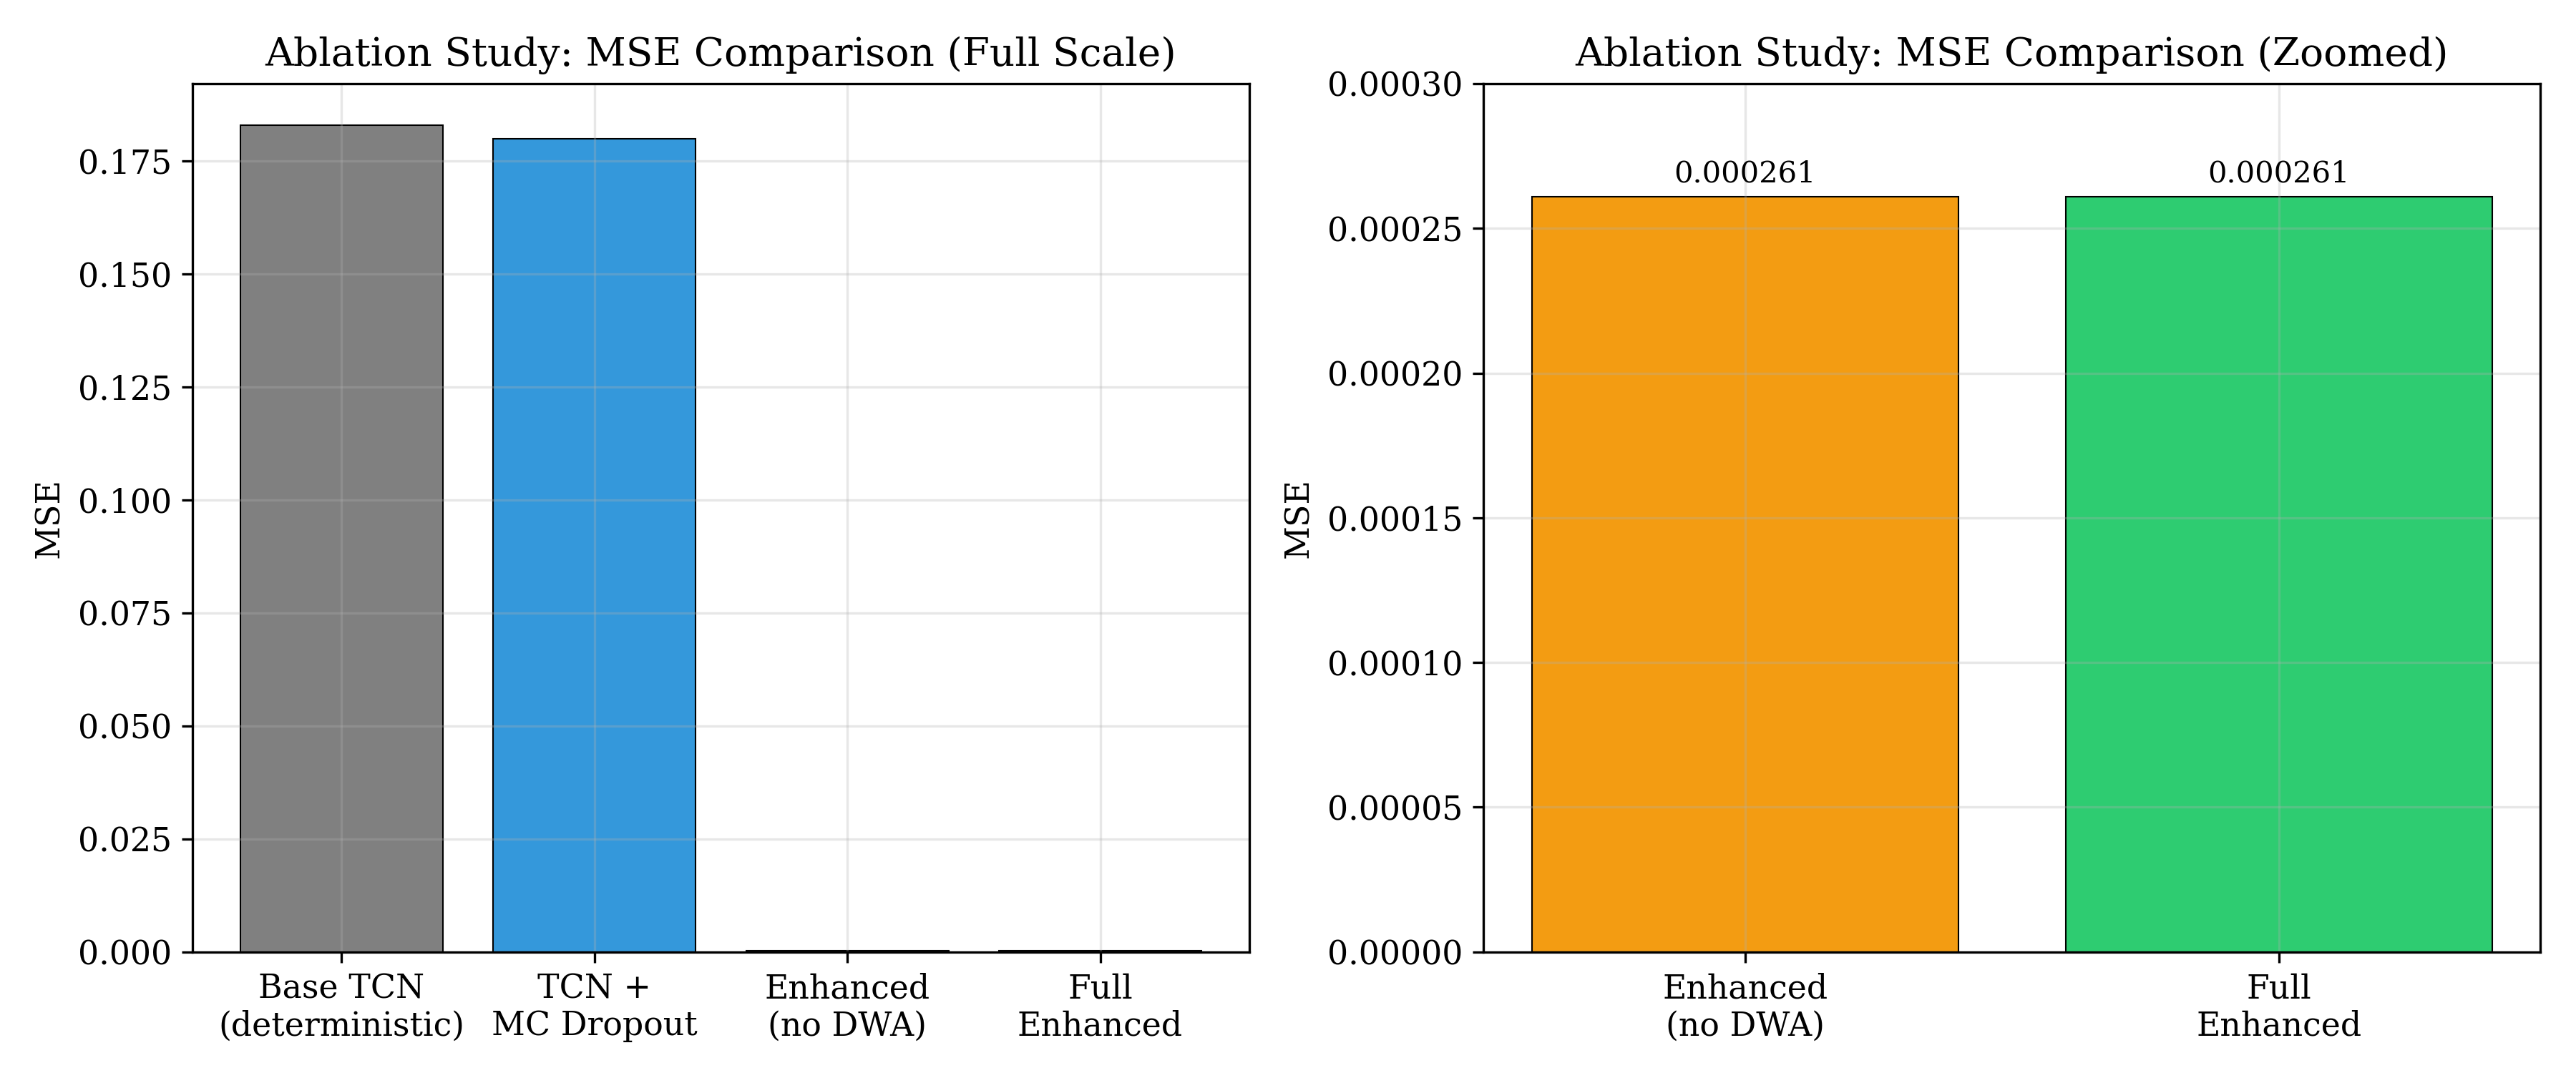
\includegraphics[width=0.85\linewidth]{images/ablation_comparison_enhanced.png}
\caption{Ablation study results. (a) Full-scale MSE comparison showing the dramatic improvement from base TCN to enhanced models. (b) Zoomed comparison between the enhanced model variants, showing that the Dynamic Weight Adapter adds negligible improvement when uncertainty is collapsed.}
\label{fig:ablation_comparison_enhanced}
\end{figure}

\begin{figure}[htbp]
\centering
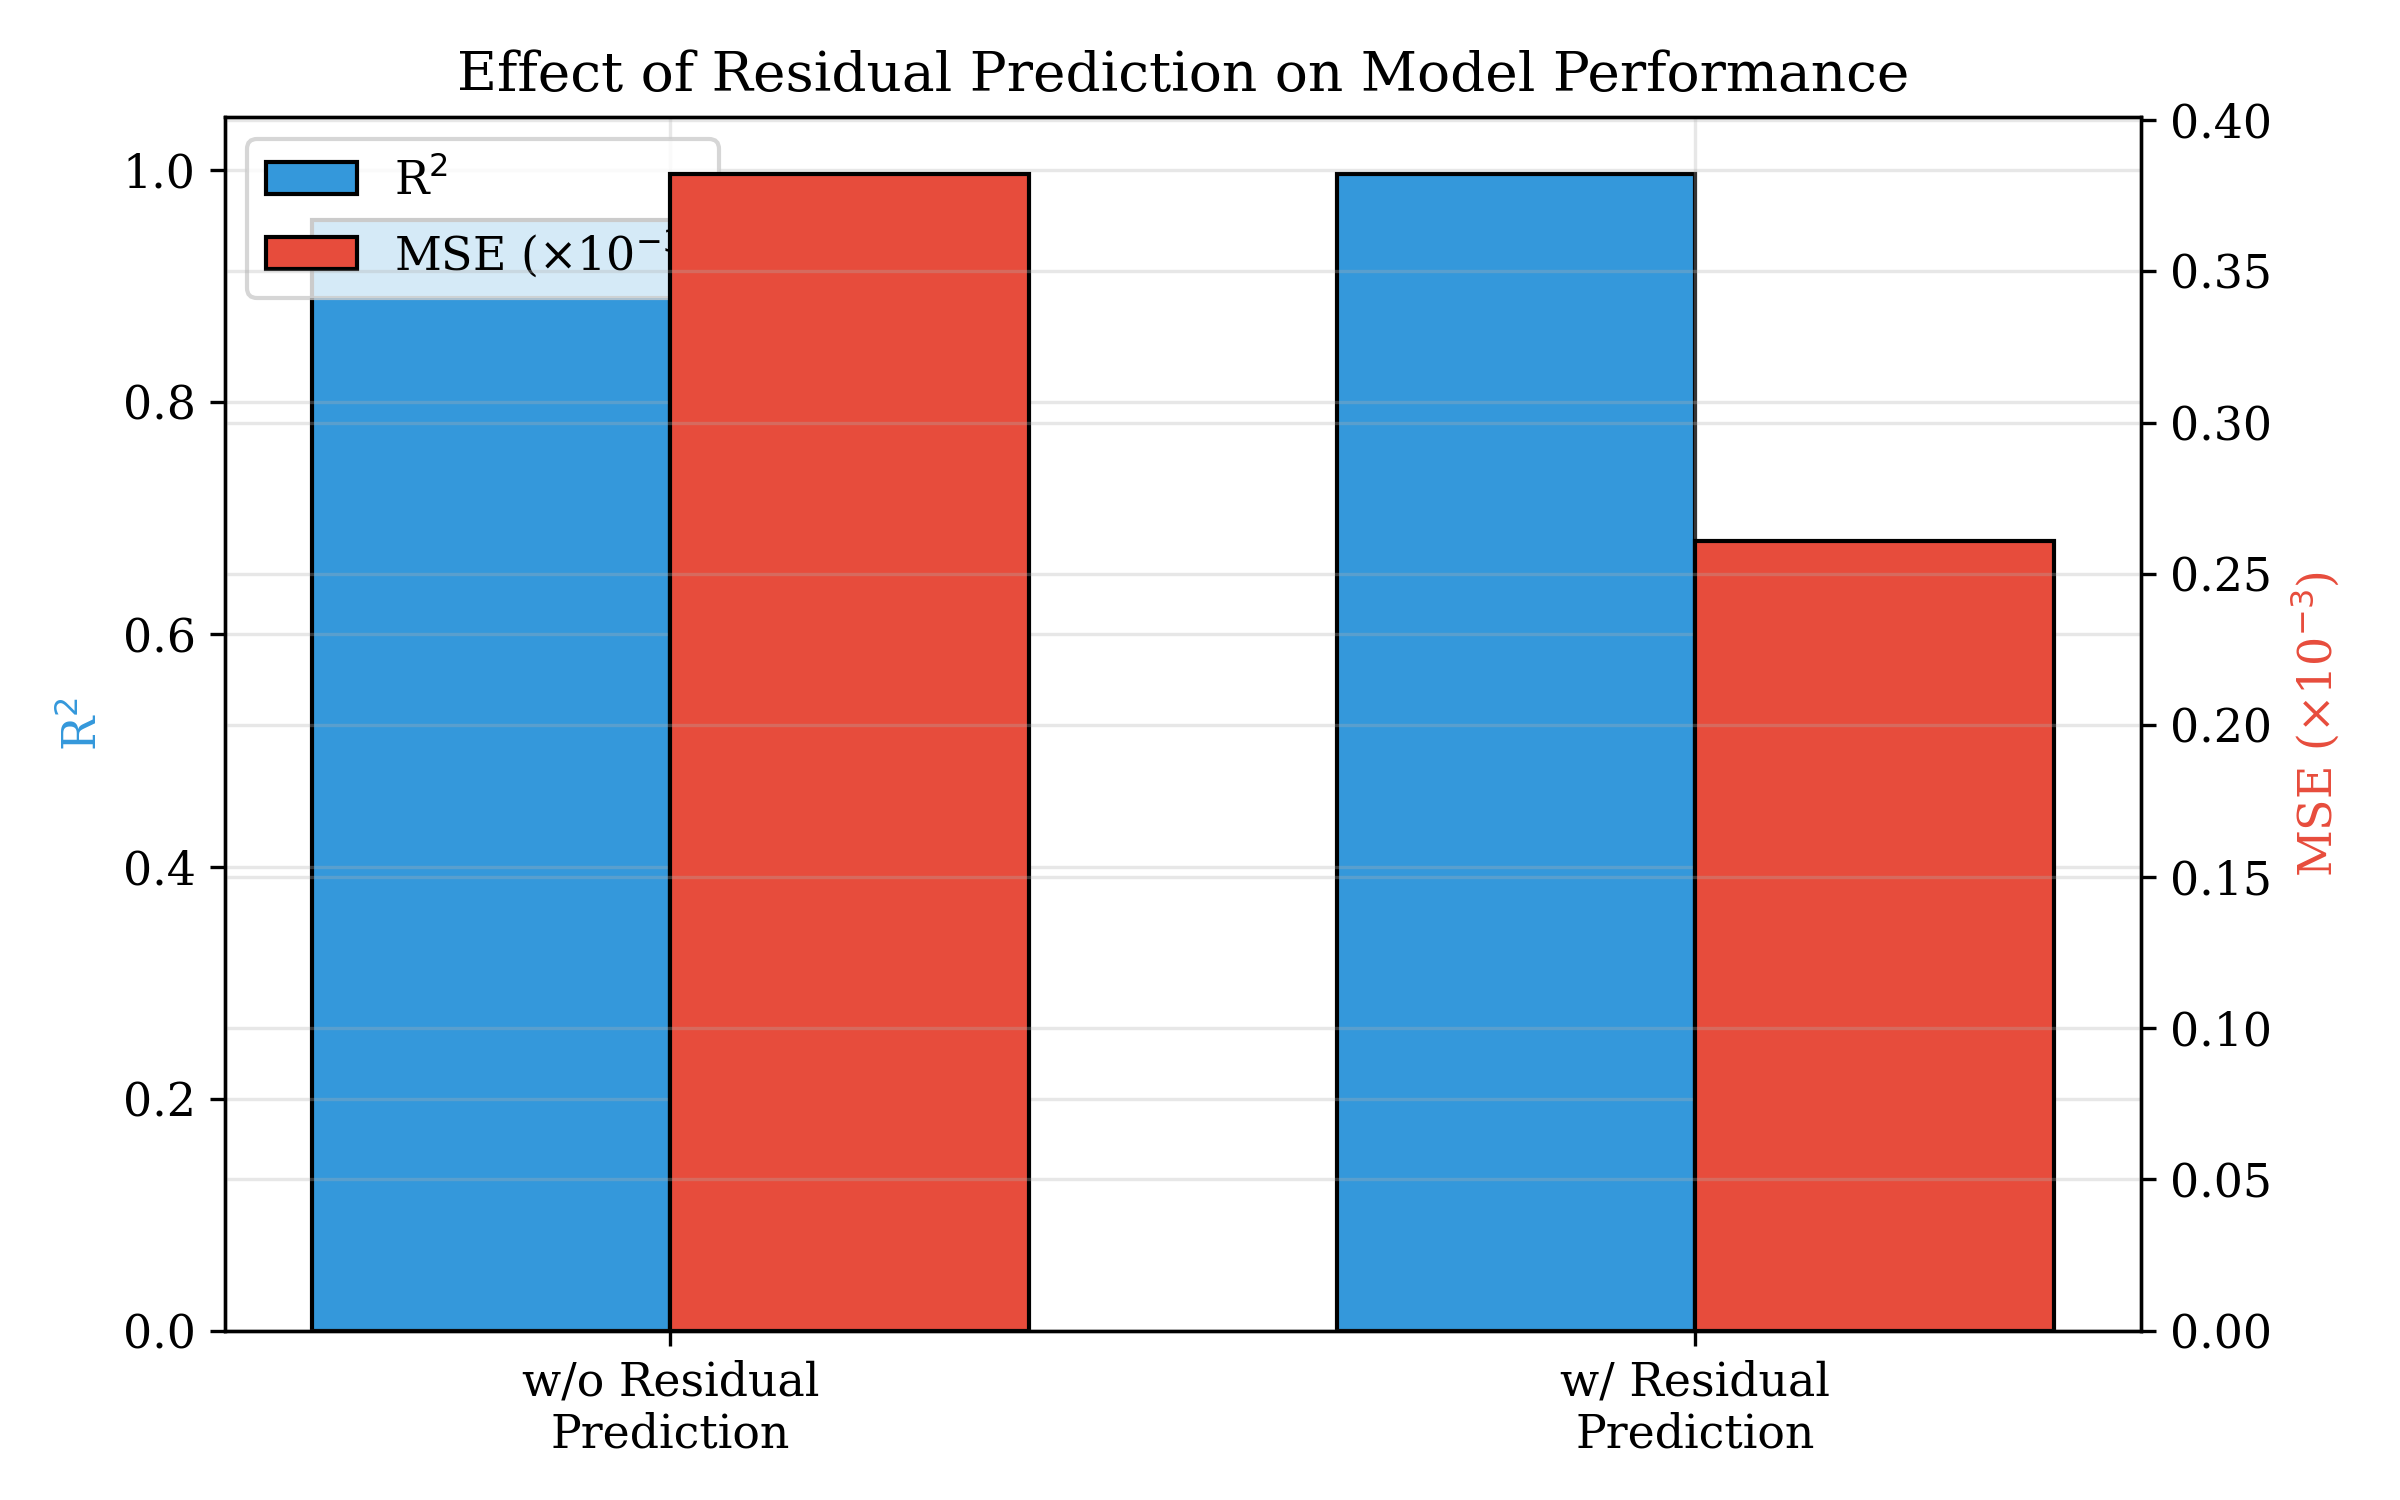
\includegraphics[width=0.7\linewidth]{images/residual_prediction_effect.png}
\caption{Effect of residual prediction on model performance. With residual prediction (predicting delta from the last timestep with zero-initialized FC), the model achieves R$^2$ = 0.9965 and MSE = 0.000261, compared to R$^2$ = 0.957 and MSE = 0.000382 without it. The residual connection provides a strong identity-like initialization that significantly accelerates convergence.}
\label{fig:residual_prediction_effect}
\end{figure}
\end{table}